\documentclass[tikz,border=2pt]{standalone}
\usepackage{amsmath,amssymb}
\usepackage{tikz}
\usetikzlibrary{matrix,arrows.meta}

\begin{document}
% Hungarian algorithm on the 3x3 example: subtract row minima, then column minima; cover the
% zeros with as few lines as possible; if fewer than n lines, subtract the smallest uncovered
% entry from the uncovered ones and add it at the crossings; repeat until a zero assignment
% of size n exists.
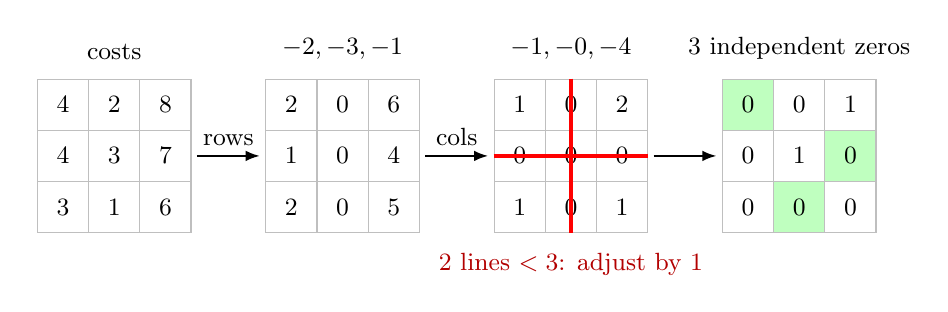
\begin{tikzpicture}[every node/.style={font=\small}, >={Latex[length=1.8mm]}]
	\matrix (A) [matrix of math nodes, nodes={minimum size=6.5mm, anchor=center, draw=gray!50}, column sep=-\pgflinewidth, row sep=-\pgflinewidth] at (0,0) {4 & 2 & 8 \\ 4 & 3 & 7 \\ 3 & 1 & 6 \\};
	\node[anchor=south] at (A.north) {costs};
	\draw[->, thick] (1.05,0) -- (1.85,0) node[midway, above] {rows};
	\matrix (B) [matrix of math nodes, nodes={minimum size=6.5mm, anchor=center, draw=gray!50}, column sep=-\pgflinewidth, row sep=-\pgflinewidth] at (2.9,0) {2 & 0 & 6 \\ 1 & 0 & 4 \\ 2 & 0 & 5 \\};
	\node[anchor=south] at (B.north) {$-2,-3,-1$};
	\draw[->, thick] (3.95,0) -- (4.75,0) node[midway, above] {cols};
	\matrix (Cm) [matrix of math nodes, nodes={minimum size=6.5mm, anchor=center, draw=gray!50}, column sep=-\pgflinewidth, row sep=-\pgflinewidth] at (5.8,0) {1 & 0 & 2 \\ 0 & 0 & 0 \\ 1 & 0 & 1 \\};
	\node[anchor=south] at (Cm.north) {$-1,-0,-4$};
	\draw[red, very thick] (Cm-2-1.west) -- (Cm-2-3.east);
	\draw[red, very thick] (Cm-1-2.north) -- (Cm-3-2.south);
	\node[red!70!black, anchor=north] at (Cm.south) {$2$ lines $<3$: adjust by $1$};
	\draw[->, thick] (6.85,0) -- (7.65,0);
	\matrix (D) [matrix of math nodes, nodes={minimum size=6.5mm, anchor=center, draw=gray!50}, column sep=-\pgflinewidth, row sep=-\pgflinewidth] at (8.7,0) {|[fill=green!25]| 0 & 0 & 1 \\ 0 & 1 & |[fill=green!25]| 0 \\ 0 & |[fill=green!25]| 0 & 0 \\};
	\node[anchor=south] at (D.north) {$3$ independent zeros};
	\end{tikzpicture}
\end{document}
